\documentclass[12pt]{article}
\usepackage[dvips]{graphicx}
\topmargin -40pt
\headsep 30pt
\evensidemargin 0pt
\oddsidemargin 0pt
\textwidth 490pt
\textheight 650pt


\def\beq{\begin{equation}}
\def\eeq{\end{equation}}

\begin{document}

%\newpage
\section*{Verdict Tetrahedral Metrics:}

\subsection*{Variable Definitions:}

\begin{figure}[htb]
  \begin{center}
    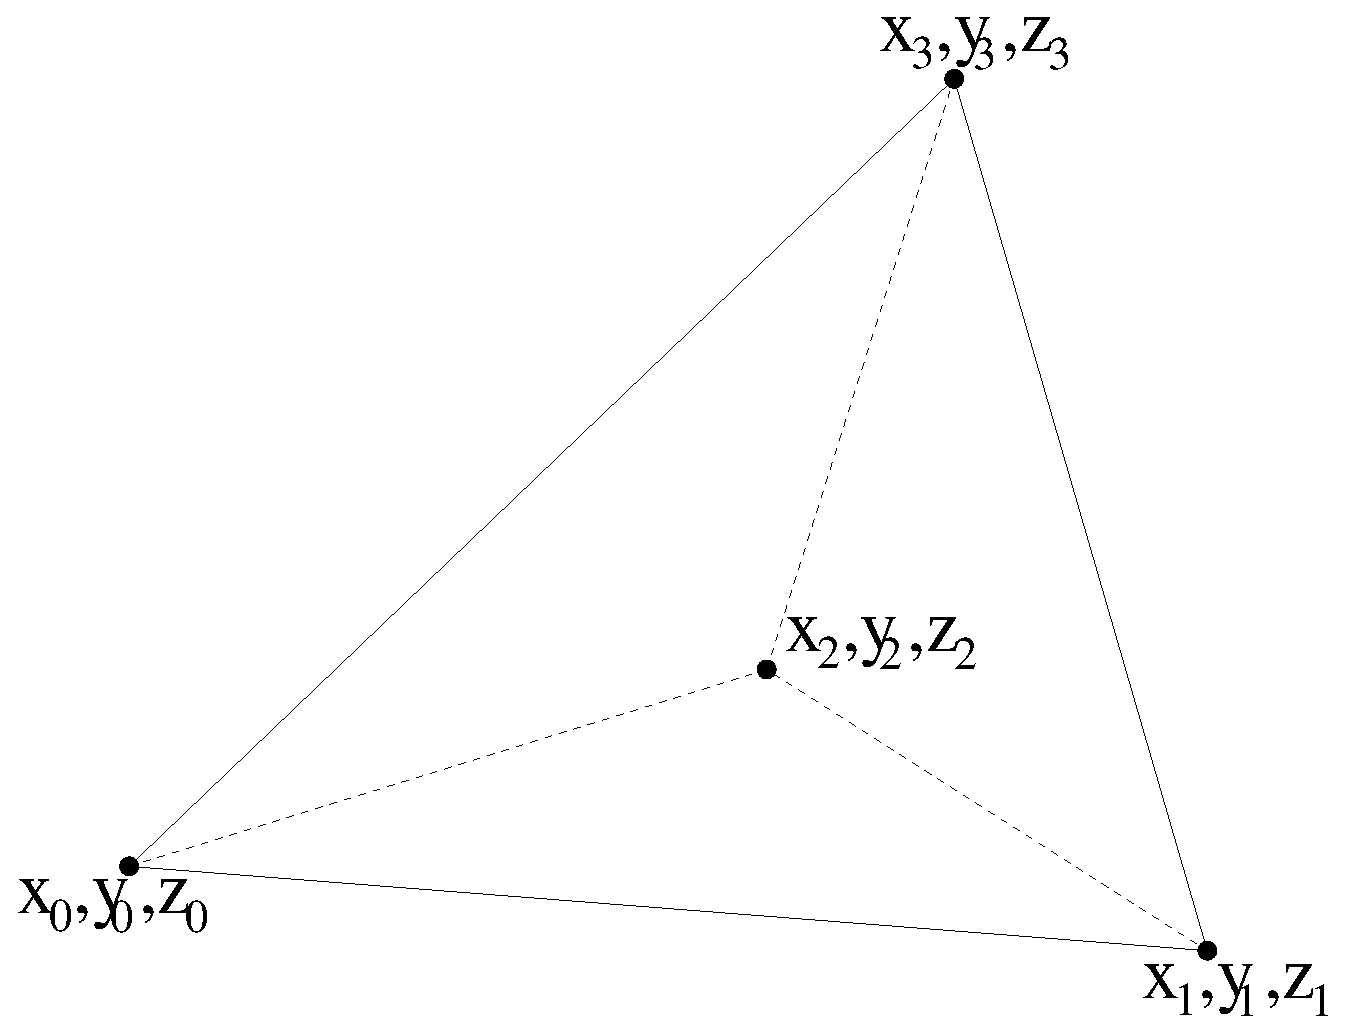
\includegraphics[height=2.0in]{tet.eps}
    \caption{Vertices of Tetrahedron. Point $P_2$ is behind face $P_0$-$P_1$-$P_3$ }
    \label{fig:blank}
  \end{center}
\end{figure}

\subsubsection*{Tet Vertices:}
\begin{center}
$\vec P_0 = (x_0, y_0, z_0)$
\end{center}

\begin{center}
$\vec P_1 = (x_1, y_1, z_1)$
\end{center}

\begin{center}
$\vec P_2 = (x_2, y_2, z_2)$
\end{center}

\begin{center}
$\vec P_3 = (x_3, y_3, z_3)$
\end{center}

\subsubsection*{Tet Edge Vectors:}

\begin{center}
$\vec L_0 = \vec P_1 - \vec P_0 $
\end{center}

\begin{center}
$\vec L_1 = \vec P_2 - \vec P_1 $
\end{center}

\begin{center}
$\vec L_2 = \vec P_0 - \vec P_2 $
\end{center}

\begin{center}
$\vec L_3 = \vec P_3 - \vec P_0 $
\end{center}

\begin{center}
$\vec L_4 = \vec P_3 - \vec P_1 $
\end{center}

\begin{center}
$\vec L_5 = \vec P_3 - \vec P_2 $
\end{center}


\beq 
V = \frac { \left( \vec L_2 \times \vec L_0 \right) \cdot \vec L_3  }  
          {6} 
\eeq

\subsection*{Metric Ranges:}

\begin{flushleft}
Acceptable Range: Well-behaved elements will have metrics in this range.
\end{flushleft}
\begin{flushleft}
Normal Range:     All elements except those with degeneracies will have  \newline
                  metrics in this range.
\end{flushleft}
\begin{flushleft}
Full Range:       All elements including degenerate ones will have metrics \newline
                  in this range. 
\end{flushleft}

\begin{flushleft}
NOTE:  The metrics below are all checked for overflow like so:
\end{flushleft}

\begin{flushleft}
${IF \quad metric\_value > 0;  \quad metric\_value = MIN( metric\_value, DBL\_MAX )}$
\end{flushleft}
 
\begin{flushleft}
${ELSE \quad metric\_value = MAX( metric\_value, -DBL\_MAX )}$
\end{flushleft}

%---------------------------Aspect Ratio Beta-----------------------------
\subsection*{Tet Aspect Ratio Beta:}

\begin{displaymath}
Area_{surface} = \frac{1}{2} * \left(
                    |\vec L_2 \times \vec L_0| + 
                    |\vec L_3 \times \vec L_0| + 
                    |\vec L_4 \times \vec L_1| + 
                    |\vec L_3 \times \vec L_2|  \right)
\end{displaymath}

\begin{displaymath}
 Rad_{inscribed} = \frac { 3V } { Area_{surface} }
\end{displaymath}

\begin{displaymath}
 Rad_{circum} = \frac {\left| 
                              |\vec L_3|^2 * \vec L_2 \times \vec L_0 + 
                              |\vec L_2|^2 * \vec L_3 \times \vec L_0 + 
                              |\vec L_0|^2 * \vec L_3 \times \vec L_2 
                              \right|
                              }
                              {12 * V } 
\end{displaymath} 

\begin{eqnarray}
aspect~ratio~beta & = & \frac { Rad_{circum} } {3*Rad_{inscribed} } \nonumber 
\\
                  & = &\frac { \left| 
                             |\vec L_3|^2 * \vec L_2 \times \vec L_0 + 
                             |\vec L_2|^2 * \vec L_3 \times \vec L_0 + 
                             |\vec L_0|^2 * \vec L_3 \times \vec L_2 
                             \right| * Area_{surface} }
                            { 108V^2}
\end{eqnarray}

\begin{tabular}{lll}
& Metric Description:  & One third ratio of circumsphere radius to inscribed \\
&                      & sphere radius of tet. \\
& Dimension:           & $L^0$              \\ 
& Acceptable Range:    & 1 to 3 \\ 
& Normal Range:        & 1 to $DBL\_MAX$   \\ 
& Full Range:          & 1 to $DBL\_MAX$   \\ 
& Value of Metric on   &  \\
& Unit Equilateral Tetrahedron:    & 1.0 \\
& Note:                & If $|V| < DBL\_MIN$, $aspect~ratio~beta = DBL\_MAX$ \\
& Reference:           &  \cite{one} \\
\end{tabular} 



%---------------------------Aspect Ratio Gamma-----------------------------
\subsection*{Tet Aspect Ratio Gamma:}

\begin{displaymath}
R = \sqrt{ \frac{ |\vec L_0|^2 + |\vec L_1|^2 + 
                  |\vec L_2|^2 + |\vec L_3|^2 + 
                  |\vec L_4|^2 + |\vec L_5|^2  } {6} }
\end{displaymath}

\begin{displaymath}
aspect~ratio~gamma = \frac{R^3}{|V|}\frac{\sqrt{2}}{12}
\end{displaymath}

\begin{tabular}{lll}
& Metric Description:  & Normalized ratio of root-mean-square \\ 
&                      & edge-length cubed to tet volume. \\
& Dimension:           & $L^0$              \\ 
& Acceptable Range:    & 1 to 3 \\ 
& Normal Range:        & 1 to $DBL\_MAX$   \\ 
& Full Range:          & 1 to $DBL\_MAX$   \\ 
& Value of Metric on   &  \\
& Unit Equilateral Tetrahedron:    & 1.0 \\
& Note:                & If $|V| < DBL\_MIN$, $aspect~aatio~gamma = DBL\_MAX$ \\
& Reference:           & \cite{one} \\
\end{tabular} 



%---------------------------Condition-----------------------------
\subsection*{Tet Condition Number:}

\begin{displaymath}
\vec C_1 = \vec L_0 
\end{displaymath}

\begin{displaymath}
\vec C_2 = \frac {-2 * \vec L_2 - \vec L_0} { \sqrt{3} } 
\end{displaymath}

\begin{displaymath}
\vec C_3 = \frac {3 * \vec L_3 + \vec L_2 - \vec L_0 } { \sqrt{6} }
\end{displaymath}

\begin{displaymath}
T_1 = C_1 \cdot C_1 + C_2 \cdot C_2 + C_3 \cdot C_3
\end{displaymath}

\begin{displaymath}
T_2 = (C_1 \times C_2 ) \cdot (C_1 \times C_2) + 
      (C_2 \times C_3 ) \cdot (C_2 \times C_3) + 
      (C_1 \times C_3 ) \cdot (C_1 \times C_3)  
\end{displaymath}

\begin{displaymath}
det = \vec C_1 \cdot ( \vec C_2 \times \vec C_3 ) 
\end{displaymath}


\begin{displaymath}
condition = \frac{ \sqrt{ T_1 * T_2 } } { 3*det } 
\end{displaymath}


\begin{tabular}{lll}
& Metric Description:  & Condition number of the Jacobian matrix at any corner  \\
&                      & referenced to a unit equilateral tetrahedron. \\ 
& Dimension:           & $L^0$  \\
& Acceptable Range:    & 1 to 3 \\ 
& Normal Range:        & 1 to $DBL\_MAX$ \\ 
& Full Range:          & 1 to $DBL\_MAX$ \\ 
& Value of Metric on   &  \\
& Unit Equilateral Tetrahedron:    & 1.0 \\
& Note:                & If $det \leq DBL\_MIN$, $condition = DBL\_MAX$  \\
& Reference:           & \cite{two} \\
\end{tabular} 



%---------------------------Distortion---------------------------
\subsection*{Hex Distortion:} 

\begin{displaymath}
distortion = \frac{ det(J)*master\textrm{-}volume} { true\textrm{-}volume }  
\end{displaymath}

\begin{flushleft} Where, \end{flushleft}
$det(J) = $ minimum determinant of the Jacobian computed over all Gauss points  \newline
of the element.  The location of the Gauss points is not documented. \newline 
\newline
$master\textrm{-}volume =$ volume of the master tet, where the master tet's corner \newline
nodes are as follows: \newline


 $\vec P_0 = ( -1, -\frac {\sqrt{3}}{3}, -\frac{ 2\sqrt{6} }{9} )$, 
 $\vec P_1 = ( 1, -\frac{\sqrt{3}}{3},  -\frac{ 2\sqrt{6} }{9} )$,
 $\vec P_2 = ( 0, \frac{2\sqrt{3}}{3},   -\frac{ 2\sqrt{6} }{9} )$,
 $\vec P_3 = ( 0, 0,   \frac{ 4\sqrt{6} }{9} )$ \newline

\begin{flushleft}  
$true\textrm{-}volume = V $ \newline
\end{flushleft}  

\begin{tabular}{lll}
& Metric Description:  & Minimum Gauss Point Jacobian divided by tet \\
&                      & volume, times master tet's volume. \\ 
& Dimension:           & $L^0$       \\ 
& Acceptable Range:    & 0.5 to 1 \\ 
& Normal Range:        & 0 to 1 \\ 
& Full Range:          & $-DBL\_MAX$ to $DBL\_MAX$ \\ 
& Value of Metric on   &  \\
& Unit Equilateral Tetrahedron:    & 0 \\
& Note:                & This metric is currently unsupported. \\ 
&                      & If $V < DBL\_MIN$, $distortion = DBL\_MAX$ \\ 
& Reference:           & Adapted from \cite{four} \\
\end{tabular} 


%---------------------------Jacobian-----------------------------
\subsection*{Tet Jacobian:}

\begin{displaymath}
jacobian = \left( \vec L_2 \times \vec L_0 \right) \cdot \vec L_3  
\end{displaymath}

\begin{tabular}{lll}
& Metric Description:  & Six times the tet volume. \\
& Dimension:           & $L^3$  \\ 
& Acceptable Range:    & 0 to $DBL\_MAX$ \\ 
& Normal Range:        & 0 to $DBL\_MAX$ \\ 
& Full Range:          & $-DBL\_MAX$ to $DBL\_MAX$                       \\ 
& Value of Metric on   &  \\
& Unit Equilateral Tetrahedron:    & $\frac { \sqrt{2} } {2} $ \\
& Reference:           & \cite{two} \\
\end{tabular} 


%---------------------------Relative Size-----------------------------
\subsection*{Tet Relative Size-Squared:}


\begin{displaymath}
R = \frac{V} {Average~Tet~Volume}
\end{displaymath}

\begin{displaymath}
relative~size \textrm{-}squared =  [ MIN( R, \frac {1}{R}) ]^2
\end{displaymath}

\begin{flushleft}
$Average ~ Tet ~ Volume$  is the average volume of the tets in the \\
group of tets being analyzed. \\
\end{flushleft}

\begin{tabular}{lll}
& Metric Description:  & Square of minimum of the ratio of tet volume to  \\
&                      & average tet volume and the inverse ratio.\\
& Dimension:           & $L^0$  \\ 
& Acceptable Range:    & 0.3 to 1 \\ 
& Normal Range:        & 0 to 1\\ 
& Full Range:          & 0 to 1 \\ 
& Value of Metric on   &  \\
& Unit Equilateral Tetrahedron:    & Depends on $Average ~ Tet ~ Volume$ \\
& Note:                & If $Average~Tet~Volume < DBL\_MIN,$  \\
&                      & $relative~size \textrm{-}squared = 0$ \\ 
&                      & If $R \leq DBL\_MIN; relative~size \textrm{-}squared = 0$ \\
& Reference:           & \cite{three} \\
\end{tabular} 

%---------------------------Scaled Jacobian-----------------------------
\subsection*{Tet Scaled Jacobian:}

\begin{displaymath}
\lambda_1 = \left| \vec L_0 \right| *
            \left| \vec L_2 \right| * 
            \left| \vec L_3 \right|  
\end{displaymath}

\begin{displaymath}
\lambda_2 = \left| \vec L_0 \right| *
            \left| \vec L_1 \right| * 
            \left| \vec L_4 \right|  
\end{displaymath}

\begin{displaymath}
\lambda_3 = \left| \vec L_1 \right| *
            \left| \vec L_2 \right| * 
            \left| \vec L_5 \right|  
\end{displaymath}

\begin{displaymath}
\lambda_4 = \left| \vec L_3 \right| *
            \left| \vec L_4 \right| * 
            \left| \vec L_5 \right|  
\end{displaymath}


\begin{displaymath}
              \lambda_{max} = MAX \left( \lambda_1, \lambda_2, \lambda_3, \lambda_4, jacobian \right) 
\end{displaymath}

\begin{displaymath}
            scaled~jacobian = \frac {\sqrt{2} * jacobian } 
                                     { \lambda_{max} }
\end{displaymath}


\begin{tabular}{lll}
& Metric Description:  & Tet Jacobian divided by the lengths of the 3 edge vectors. \\
& Dimension:           & $L^0$  \\ 
& Acceptable Range:    & $0.5$ to $1.414$ \\ 
& Normal Range:        & $-1.414$ to $1.414$\\ 
& Full Range:          & $-DBL\_MAX$ to $DBL\_MAX$\\ 
& Value of Metric on   &  \\
& Unit Equilateral Tetrahedron:    & 1.0 \\ 
& Note:                & If $ \lambda_{max} < DBL\_MIN$,  \\
&                      & $scaled~jacobian = DBL\_MAX$ \\
& Reference:           & \cite{two} \\
\end{tabular} 


%---------------------------Shape-----------------------------
\subsection*{Tet Shape:}

\begin{displaymath}
shape =  \frac{ 3 * \left( jacobian \sqrt{2} \right)^{2/3} } 
              { \frac {3}{2} \left( 
                      \vec L_0 \cdot  \vec L_0 +
                      \vec L_2 \cdot  \vec L_2 +
                      \vec L_3 \cdot  \vec L_3  \right) - 
               \left( \vec L_0 \cdot -\vec L_2 +
                      \vec L_0 \cdot  \vec L_3 +
                     -\vec L_2 \cdot  \vec L_3 \right) } 
\end{displaymath}

\begin{tabular}{lll}
& Metric Description:  & 3/Condition number of Jacobian matrix referenced to an \\
&                      & equilateral tetrahedron. \\
& Dimension:           & $L^0$  \\ 
& Acceptable Range:    & 0.3 to 1 \\ 
& Normal Range:        & 0 to 1 \\ 
& Full Range:          & 0 to 1 \\ 
& Value of Metric on   &  \\
& Unit Equilateral Tetrahedron:    & 1.0 \\ 
& Note:                & If $jacobian < DBL\_MIN$, $shape = 0$  \\
&                      & If $\frac {3}{2} \left( \vec L_0 \cdot \vec L_0 +
                      \vec L_2 \cdot \vec L_2 +
                      \vec L_3 \cdot \vec L_3  \right) - $ \\
&                      & $\left( \vec L_0 \cdot -\vec L_2 +
                      \vec L_0 \cdot \vec L_3 +
                      -\vec L_2 \cdot \vec L_3 \right) < DBL\_MIN,$ $shape = 0$ \\
& Reference:           & \cite{three} \\
\end{tabular} 


%---------------------------Shape and Size-----------------------------
\subsection*{Quad Shape and Size:}

\begin{displaymath}
shape~and~size = shape * relative~size \textrm{-}squared 
\end{displaymath}

\begin{tabular}{lll}
& Metric Description:  & Product of Shape and Relative Size Squared.\\ 
& Dimension:           & $L^0$       \\ 
& Acceptable Range:    & 0.2 to 1 \\ 
& Normal Range:        & 0 to 1 \\ 
& Full Range:          & 0 to 1 \\ 
& Value of Metric on   &  \\
& Unit Equilateral Tetrahedron:    & 1.0 \\ 
& Reference:           & \cite{three} \\
\end{tabular} 

%---------------------------Volume-----------------------------
\subsection*{Tet Volume:}

\begin{displaymath}
volume = V 
\end{displaymath}

\begin{tabular}{lll}
& Metric Description:  & One sixth determinant of jacobian at any node. \\ 
& Dimension:           & $L^3$                   \\ 
& Acceptable Range:    & 0 to $DBL\_MAX$ \\ 
& Normal Range:        & $-DBL\_MAX$ to $DBL\_MAX$   \\ 
& Full Range:          & $-DBL\_MAX$ to $DBL\_MAX$   \\ 
& Value of Metric on   &  \\
& Unit Equilateral Tetrahedron:    & $\frac { \sqrt{2}} {12} $ \\
& Reference:           & \cite{one} \\
\end{tabular} 

\begin{thebibliography}{99}

\bibitem{one}  V. N. Parthasarathy et al, A comparison of tetrahedron quality 
measures, Finite Elem. Anal. Des., Vol 15(1993), 255-261.

\bibitem{two} P. Knupp, Achieving Finite Element Mesh Quality via 
Optimization of the Jacobian Matrix Norm and Associated Quantities,
Intl. J. Numer. Meth. Engng. 2000, 48:1165-1185.

\bibitem{three} P. Knupp, Algebraic Mesh Quality Metrics for Unstructured 
Initial Meshes, Finite Elements in Analysis and Design, Vol. 39, p217-241,
2003.

\bibitem{four} SDRC/IDEAS Simulation: Finite Element Modeling--User's Guide

\end{thebibliography}

\end{document}
